\documentclass[10pt]{beamer}
%\usepackage[T1]{fontenc} DO NOT ENABLE THIS!!!

\usetheme[progressbar=frametitle]{metropolis}
\usepackage{appendixnumberbeamer}
\setbeamertemplate{footline}{}
\setbeamertemplate{navigation symbols}[horizontal]

\setbeamertemplate{title page}{
    \begin{minipage}[c][\paperheight]{\textwidth}
        \ifx\inserttitlegraphic\@empty\else\usebeamertemplate*{title graphic}\fi
        \vfill%
        \ifx\inserttitle\@empty\else\usebeamertemplate*{title}\fi
        \ifx\insertsubtitle\@empty\else\usebeamertemplate*{subtitle}\fi
        \usebeamertemplate*{title separator}
        \begin{minipage}[t]{\textwidth}
            \ifx\beamer@shortauthor\@empty\else\usebeamertemplate*{author}\fi
            \ifx\insertdate\@empty\else\usebeamertemplate*{date}\fi
            \ifx\insertinstitute\@empty\else\usebeamertemplate*{institute}\fi
        \end{minipage}
        \vfill
        \vspace*{1mm}
    \end{minipage}
}

\metroset{sectionpage=none}
\setbeamertemplate{section in toc}[sections numbered]
\setbeamertemplate{subsection in toc}[subsections numbered]


\usepackage{booktabs}
\usepackage[scale=2]{ccicons}

\usepackage{amsmath, amsfonts}

\usepackage{float}

\usepackage{tabularx}
\usepackage{booktabs}

\usepackage{xcolor}
\definecolor{linkcolour}{rgb}{0,0.2,0.6}

\usepackage{hyperref}
\hypersetup{pdfauthor={Li, Binghuan}, 
            colorlinks,breaklinks,urlcolor=linkcolour, linkcolor=linkcolour}

\title{Implementation of Boundary Conditions and The algebraic Equation System}
\subtitle{Finite Difference Method\cite{Ferziger2002}}
\author{Binghuan W Li \ $\lvert$ \   \href{mailto:binghuan.li19@imperial.ac.uk}{binghuan.li19@imperial.ac.uk}}
\institute{Department of Bioengineering, Imperial College London}
\titlegraphic{
\includegraphics[width=0.3\textwidth]{imgs/Imperial.eps}}


%================================================
\begin{document}
\maketitle
%================================================
\begin{frame}{Contents}
\tableofcontents
\end{frame}
%================================================
\section{Implementation of Boundary Conditions}
\begin{frame}{Implementation of Boundary Conditions (1/)}
Types of boundary conditions:
\begin{itemize}
    \item \textbf{Dirichlet boundary conditions:} the value of the variable at the boundary
    \item \textbf{Neumann boundary conditions:} the gradient in particular direction, usually normal to the boundary
    \item A mix of two
\end{itemize}
\end{frame}
%================================================
\begin{frame}{Implementation of Boundary Conditions(2/)}
When higher-order approximations of the derivatives are used, since they require data at more than 3 points, approximations at at interior nodes may demand data at points beyond the boundary. It may then be necessary to use different approximations to for the derivatives at points close to the boundary; usually these are of lower order than the approximations used in the interior and may be one-sided difference. \newline \newline
For Example, fitting a 4\textsuperscript{th}-order polynomial through the boundary and four inner points, the following approximation for the first derivative results at $x=x_{2}$, the first interior point:
    \[
    \bigg( \frac{\partial \phi}{\partial x}\bigg)_{2} = 
    \frac{-\phi_{5}+6\phi_{4}+18\phi_{3}+10\phi_{2}-33\phi_{1}}{60\Delta x} + \mathcal{O}((\Delta x)^{4})
    \]
Approximation of the second derivative using the same polynomial gvies:
    \[
    \bigg( \frac{\partial^{2} \phi}{\partial x^{2}}\bigg)_{2} = \frac{-21\phi_{5}+96\phi_{4}+18\phi_{3}-240\phi_{2}+147\phi_{1}}{180(\Delta x)^2} + \mathcal{O}((\Delta x)^{3})
    \]
\end{frame}
%================================================
\begin{frame}{Implementation of Boundary Conditions(3/)}
If the gradient is prescribed at the boundary, a suitable one-sided FD approximation for it can be used to compute the boundary value of the variable.\newline \newline
For example, zero gradient at the normal direction is prescribed:
    \[
    \bigg( \frac{\partial \phi}{\partial x}\bigg)_{1} = 0 \quad \Rightarrow \quad \frac{\phi_{2}-\phi_{1}}{x_{2}-x_{1}} = 0 \quad \Rightarrow \quad \phi_{2} = \phi_{1}  
    \]
From a parabolic fit to the boundary and two inner points, the following second-order approximation is obtained for the first derivative at the boundary:
    \[
    \bigg( \frac{\partial \phi}{\partial x}\bigg)_{1} \approx \frac{-\phi_{3}(x_{2}-x_{1})^2 + \phi_{2}(x_{3}-x_{1})^{2} - \phi_{1}[(x_{3}-x_{1})^{2}-(x_{2}-x_{1})^{2}]}{(x_{2}-x_{1})(x_{3}-x_{1})(x_{3}-x_{2})}
    \]
On a uniform grid:
    \[
    \bigg( \frac{\partial \phi}{\partial x}\bigg)_{1} \approx \frac{-\phi_{3}+4\phi_{2}-3\phi_{1}}{2\Delta x}
    \]
\end{frame}
%================================================
\begin{frame}{Implementation of Boundary Conditions(4/)}
A 3\textsuperscript{rd}-order approximation on equispaced grids is obtained from a cubic fit to four points:
    \[
     \bigg( \frac{\partial \phi}{\partial x}\bigg)_{1} \approx 
     \frac{2\phi_{4}-9\phi_{3}+18\phi_{2}-11\phi_{1}}{6\Delta x}
    \]
When the compact schemes are used, one has to provide both the variable value and the derivative at the boundary nodes. Usually, one of these is known and other must be computed using the information from the interior. On the other hand, polynomial interpolation can be used to compute the boundary value if the derivative is known. From a cubic fit to 4 points, the following expression is obtained for the boundary value:
    \[\phi_{1} = \frac{18\phi_{2}-9\phi_{3}+2\phi_{4}}{11} - \frac{6\Delta x}{11}\bigg( \frac{\partial \phi}{\partial x}\bigg)_{1}\]
\end{frame}
%================================================
\section{The Algebraic Equation System}
\begin{frame}{The Algebraic Equation System (1/)}
We consider only the \textbf{linear} differential equations. The result of discretization is a system of linear algebraic equations of the form:
    \[ A_{\mathrm{P}}\phi_{\mathrm{P}}+\sum_{l}A_{l}\phi_{l} = Q_{\mathrm{P}} \]
where 
\begin{itemize}
    \item $\mathrm{P}$ denotes the node at which the partial differential equation is approximated; The node $\mathrm{P}$ and neighbours form the so-called \emph{computational molecule}.
    \item index $l$ runs over the neighbour nodes involved in finite-difference approximations.
    \item The coefficients $A_{l}$ depend on geometrical quantities, fluid properties and for non-linear equations, the variable values themselves.
    \item $Q_{\mathrm{P}}$ contains all the terms which do not contain unknown variable values. 
\end{itemize} 
\end{frame}
%================================================
\begin{frame}{The Algebraic Equation System (2/)}
The node $\mathrm{P}$ and neighbours form the so-called \emph{computational molecule}.
\begin{figure}[H]
    \centering
    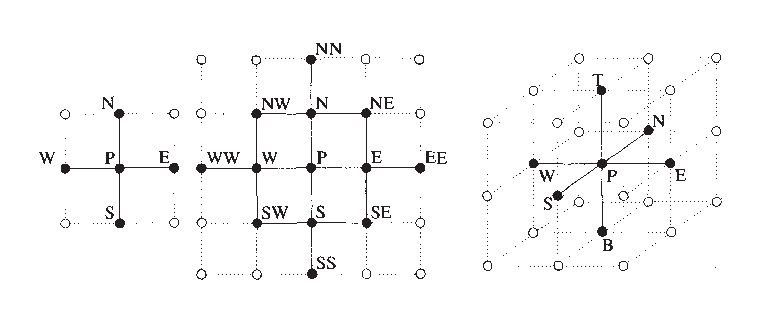
\includegraphics[width=.8\textwidth]{imgs/computational-molecules.eps}
    \caption{Examples of computational molecules in 2D and 3D}
    \label{fig:comp_mol}
\end{figure}
\end{frame}
%================================================
\begin{frame}{The Algebraic Equation System (3/)}
The numbers of equations and unknowns must be equal - one equation for each grid node. Thus we get a large set of linear algebraic equations, which must be solved numerically. The system is sparse, meaning each equation contains only few unknowns. 
    \[A\phi = \mathbf{Q}\]
where 
\begin{itemize}
    \item $A$ is the square sparse coefficient matrix, depending on the ordering of the variables in $\phi$;
    \item $\phi$ is a vector containing the variable values at the grid nodes;
    \item $\mathbf{Q}$ is the vector containing the RHS terms in $\displatstyle A_{\mathrm{P}}\phi_{\mathrm{P}}+\sum_{l}A_{l}\phi_{l} = Q_{\mathrm{P}}$.
\end{itemize} 
\end{frame}
%================================================
\begin{frame}{The algebraic Equation System (4/)}
For structured grids, if the variable are labelled staring at a corner and traversing line after line in a regular manner (lexicographic ordering), the matrix has a poly-diagonal structure.
\newline \newline
For the case of a five-point computational molecule, all the non-zero coefficient lie on the main diagonal, the two neighbour diagonals, and two other diagonal removed by $N$ positions from the main diagonal, where $N$ is the number of odes in one direction. All other coefficients are zero.
\end{frame}
%================================================
\begin{frame}{The algebraic Equation System (5/)}
For the sake of definiteness, order the entries in $\phi$ starting from the southwest corner of the domain, and processing northwards along each grid line, and then eastward across the domain. The conversion between the locations, compass notation and storage location (1-dim array in computer) are listed below.
    \begin{table}[H]
    \centering
    \begin{tabular}{lll} 
        \toprule
        Grid location   & Compass notation  & Storage location \\ 
        \midrule
        $i, j, k$   &   P   &   $l = (k-1)N_{j}N_{i}+(i-1)N_{j}+j$ \\
        $i-1, j, k$ &   W   &   $l=N_{j}$ \\
        $i, j-1, k$ &   S   &   $l-1$ \\
        $i, j+1, k$ &   N   &   $l+1$  \\
        $i+1, j, k$ &   E   &   $l+N_{j}$  \\
        $i, j, k-1$ &   B   &   $l-N_{i}N_{j}$ \\
        $i, j, k+1$ &   T   &   $l+N_{i}N_{j}$\\ 
        \bottomrule
    \end{tabular}
    \caption{Conversion of grid indices to one-dimensional storage locations for vector or column matrices}
    \label{tab:storage_location}
\end{table}
\end{frame}
%================================================
\begin{frame}{The algebraic Equation System (6/)}
Storing the elements of each non-zero diagonal in a separate array of dimension $1\times N_{i}N_{j}$, where $N_{i}$ and $N_{j}$ are the numbers of grid points in the two coordinate directions, only requires $5N_{i}N_{j}$ words of storage; Full array storage would require $N_{i}^{2}N_{j}^{2}$ words of storage. 
\newline \newline
In three dimensions, the numbers are $7N_{i}N_{j}N_{k}$ and  $N_{i}^{2}N_{j}^{2}N_{k}^{2}$.
\newline \newline
\textbf{Difference:} the diagonal-storage scheme may allow the problem to be kept in main memory when full-array scheme scheme does not.
\end{frame}
%================================================
\begin{frame}{The algebraic Equation System (7/)}\small
According to the table \autoref{tab:storage_location}, the linearized algebraic equations in two dimensions can now be written in the form
    \[
    A_{l, l-N_{j}}\phi_{l-N_{j}} + A_{l, l-1}\phi_{l-1} + A_{l,l}\phi_{l} + A_{l, l+1}\phi_{l+1} +A_{l,l+N_{j}}\phi_{l+N_{j}} = Q_{l}
    \]
\begin{figure}[H]
    \centering
    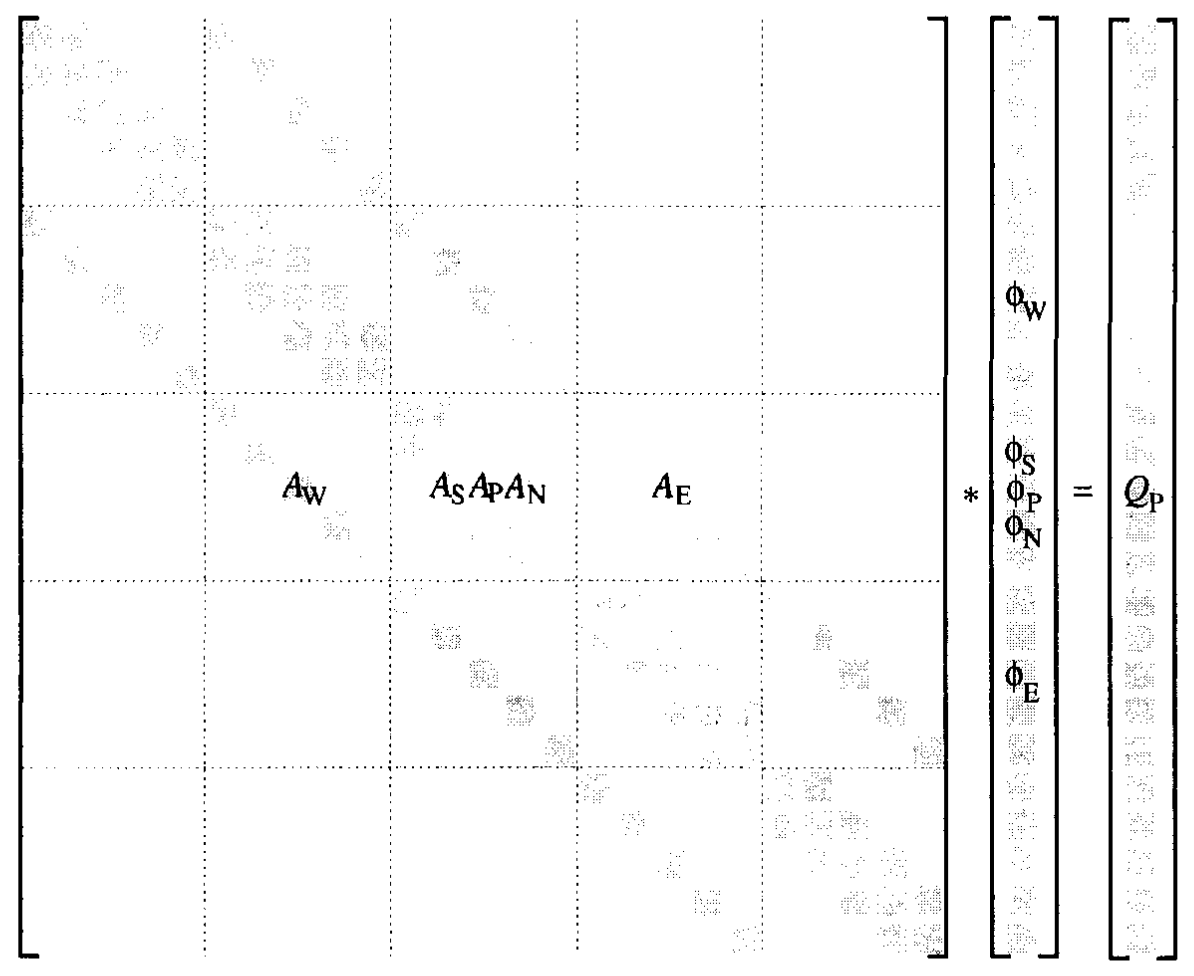
\includegraphics[width=.6\textwidth]{imgs/five-point-matrix.png}
    \caption{Structure of the matrix for a five-point computational molecule.}
    \label{fig:my_label}
\end{figure}
\end{frame}
%================================================
\appendix
\begin{frame}{Reference}
 \bibliography{bibTeX/ferziger.bib}
 \bibliographystyle{abbrv}
\end{frame}
%================================================
\end{document}
